\documentclass[10pt]{./IEEEtran}


\usepackage{cite}
\usepackage[pdftex]{graphicx}
\usepackage{amsmath}
\usepackage{mathrsfs}


\begin{document}


\title{Federation Among Remote Military Data Stores In Austere Environments}

\author{\IEEEauthorblockN{Steven Mazza}\\
\IEEEauthorblockA{School of Systems Engineering\\
Naval Postgraduate School\\
Monterey, CA 93943\\
Email: spmazza@nps.edu}}


\maketitle


\begin{abstract}
Transportable computing and some degree of network connectivity have been a necessary component of US military operations at least since the advent of the personal computer in the 1980s.  Subsequent ubiquity of laptop computers and, more recently, hand held devices such as the smart phone have exacerbated the situation by allowing the need for data and the locus of computing power to be increasingly distributed and fragmented.  Through model design and discussion we address some aspects of one potential solution to this fragmentation through federation of data stores.  In particular, we show that we are likely to obtain eventual consistency of data, even in austere environments.  Furthermore, we show that we can improve on the worst case for the time in which this state can be achieved, $O(n^{2})$ where $n$ is the number of nodes in the network.  By altering the network topology by introducing temporary cycles with varying degrees of probability, we approach time proportional to $O(log(n))$ in the best case and $O(n)$ in the average.
\end{abstract}


\IEEEpeerreviewmaketitle


\section{Introduction}
\label{sec:introduction}
Transportable computing and some degree of network connectivity have been a necessary component of US military operations at least since the advent of the personal computer in the 1980s.  Subsequent ubiquity of laptop computers and, more recently, hand held devices such as the smart phone have exacerbated the situation by allowing the need for data and the locus of computing power to be increasingly distributed and fragmented.  

Consequently, there exists a significant and growing problem related to the decentralization of computing in the United States military.  Due to the increasing distribution of computing power and data storage, there is now an acknowledged need to implement some form of federation\cite{Takai:2012} in order to maintain data concurrency.  This is especially true in theaters of operation that are characterized as austere environments and for which communications are assumed to be disconnected, intermittent, or limited (DIL), and where connections to a centralized data store are impractical or impossible\cite{Sonnenberg:2009}.

The paper is structured as follows.  We begin in Section \ref{sec:probspace} by introducing the problem space, which includes a discussion of the motivation for this work along with the questions we address.  Section \ref{sec:doe} sets up the design of experiments that we use to address the questions introduced in Section \ref{sec:probspace}.  Next we dive into a discussion of the model design in Section \ref{sec:model}.  We discuss the model development and constraints including bandwidth and connectivity, edge construction, and graph topology.  Disaster recovery is briefly related to our study in Section \ref{sec:dr}, and we wrap up with related work in Section \ref{sec:related} and finally a conclusion in Section \ref{sec:conclusion}.


\section{Problem Space}
\label{sec:probspace}
United States involvement in military operations over the past fifteen years has been in operationally challenging environments.  Lack of existing infrastructure to provide necessary operational support has been a primary challenge to sustaining long-term presence necessary to achieve our national security goals.  We focus on the challenges associated with fighting in an asymmetrical conflict while operating in an environment in which the transmission of electronic data is challenging at best.

\subsection{Motivation}
Maintaining data consistency in support of military operations is an important component to ensuring that everyone is working from the same basis of understanding in carrying out the Commander's intent.\footnote{Commander's intent in the military context is the broad context under which both direction is given by 06 officers and specific actions are taken by MAJ and SGT warfighters.}  If a given unit in formation is working off of a differential of understanding due either to stale or missing data, that unit runs the risk of inadvertently placing others in harm's way.

Data can be relatively immutable and persist for long periods of time, as with terrain maps which tend to change little over the course of conflict.  On the other hand much of the important data is highly volatile and often takes the form of overlays on tactical maps.  Data such as current friendly force and enemy positions, locations of supply and weapons cache, and route planning characterize this type of data.  Intelligence data, recent significant events, and UAS feeds all have a relatively short shelf life and tend to get updated frequently.

This more volatile type of data is typical of that which is both produced and consumed by many programs of record (PoRs).\footnote{Examples in the US Army include Command Post of the Future (CPoF) and Joint Battle Command Platform (JBC-P)}  Programs of record refer to systems that are fielded by Program Management organizations in the Army and comprise the tools with which warfighters accomplish their jobs.  In the absence of a unified mechanism and in an effort to ensure the best information is delivered to the warfighter at any point, each of these PoRs attempts to individually address the problems of data synchronization.

This presents a problem for the military for several reasons.  On the surface, stove-piped solutions present an ongoing barrier to interoperability and compatibility.  But on a more fundamental level, there exists a commonality for the need to have access to federation as a service.  In this way the military can proactively protect and manage bandwidth as an organizational resource.  We want to view bandwidth, for example, as a resource and treat it similarly to ammunition and fuel.


\subsection{Questions}
Here is what we intend to address.  We would like to know if we can guarantee the eventual consistency of data, if even statistically.  Furthermore, we would like to know in what sort of time can we expect to achieve data consistency. For the investigation of these concerns we will address time as a function of algorithmic complexity\footnote{We express complexity in big O notation.}, although that could easily be extrapolated to an estimate of elapsed time.


\section{Design of Experiments}
\label{sec:doe}
We begin by constructing an acyclic undirected graph as described in Section \ref{sec:model} with $n$ nodes.  We assign some $\rho$ data elements to each node, and assume unlimited capacity.  Storage is not expensive, and the cost per unit storage is dropping in excess of that predicted by Moore's Law.  Consequently, any accounting for capacity as a significant factor will be rapidly made obsolete by the market.  Furthermore, as connectivity increases, we may begin to naturally favor solutions such as a dynamic distributed federated database (DDFD) which allow queries to be distributed across the network\cite{Bent2009}.

We first measure the time steps, $t$, required to synchronize all $n$ nodes of the network with $\rho$ elements of data, and show that this operation completes in polynomial time.  Next we re-establish our initial conditions and run our experiment again with the introduction of randomly assigned edges, creating temporary cycles in the graph.  These edges can be seen in Figure \ref{fig:network} and are assigned as follows.

We select two non-adjacent nodes, $\mathscr{N}_{i}$ and $\mathscr{N}_{j}$, of the graph at random, with probability proportional to their connectivity within their respective immediate neighbors, $p(\mathscr{N}_{i})$ and $p(\mathscr{N}_{j})$, which we can refer to as $p_{i}$ and $p_{j}$ for convenience.  We allow the newly created edge to persist for one time step during which both nodes can perform a full exchange of data.  Note that it is possible, given sufficiently low probability of overall connectivity, that no new edge will be created on any given time step, $\tau_{t}$.  In fact, it is this probability with which cycles are introduced that determines the number of cycles at any step.  This ultimately determines the order of time in which we can achieve consistency among the nodes.


\section{Model Design}
\label{sec:model}
We have an interesting situation in that the physical organization of the network is highly structured, as prescribed by military doctrine, which favors a top-down, hierarchical task organization with a relatively fixed number of nodes at each echelon.  We generalize this as a tree structure in the classical sense, having no closed loops.  Then, as in Figure \ref{fig:network}, we augment this structure by introducing some loops that connect nodes both laterally and across echelons.  This represents various opportunities for data delivery and synchronization scenarios that are not uncommon to actual operational threads.

\subsection{Bandwidth and Connectivity}

Where this graph structure becomes particularly interesting is in the implementation of the edges.  Due to limited resources in most all theaters of operation\footnote{At the time of the writing of this paper, recent theaters of operation included Iran, Iraq, and Afghanistan.} we model the probability of connectivity and bandwidth as an edge weight that tends to follow an inverse power formula proportional to the distance of any node, $\mathscr{N}_{k}$, to the root node, $\mathscr{N}_{0}$.  Figure \ref{fig:probcon} shows a range of representative probabilities of connectivity that might suit a model given a variety of working environmental conditions.  We develop a plot of the probability by echelon and vary the overall likelihood by altering $n$ to suit measurable conditions.

\begin{figure}[h!]
  \centering
    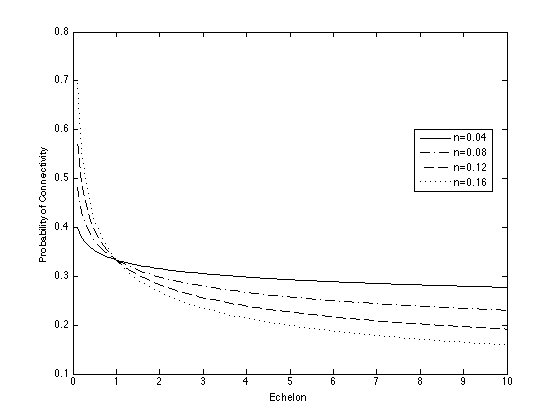
\includegraphics[width=0.5\textwidth]{images/probcon}
  \caption{Representative probabilities of connectivity by echelon, given various conditions.}
  \label{fig:probcon}
\end{figure}

We allow creation of the graph model dynamically by also using an inverse power formula to approximate bandwidth  within the constraints of our graph model.  We can see this illustrated in Figure \ref{fig:bandwidth}.  We assume distance, $d$, as the graph distance between any two given nodes, $\mathscr{N}_i$ and $\mathscr{N}_j$ such that $d(\mathscr{N}_{i}, \mathscr{N}_{j})$ is the geodesic distance with $0<d\leq \epsilon(v)$, where $\epsilon(v)$ is the graph diameter.  We construct the graph following this basic model but adjust the values, $K$ and $\lambda$, to allow a correction for the particular constraints of any specific environment.
\[
	p(\mbox{connectivity}) = \dfrac{1}{Kn_{k}^{\lambda n}}
\]

\begin{figure}[h!]
  \centering
    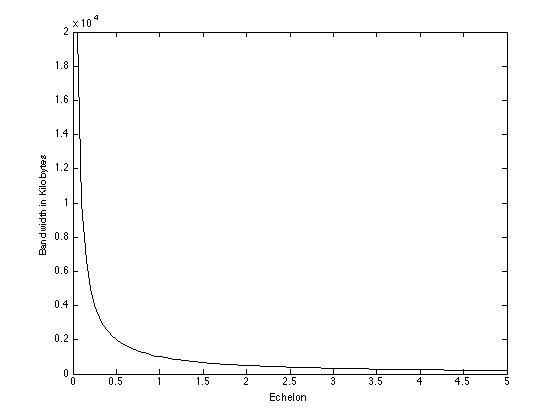
\includegraphics[width=0.5\textwidth]{images/bandwidth}
  \caption{Example representation of bandwidth by echelon.}
  \label{fig:bandwidth}
\end{figure}

\subsection{Undirected Graph}
While the traditional flow of information in a military hierarchy follows a top-down model, we implement an undirected graph.  We feel this is in keeping with the stated specific desire that each soldier become a sensor on the network\cite{Patton:2003}.  A direct result of this is that information will naturally flow naturally both up and down the traditional chain of command.  An unintended consequence is that, due largely to task re-organization, general officer and staff mobility, and transient network connections, it may also flow laterally within a structural organization and even across formations.  We will further see how this occasional lateral flow of information facilitates our desired end state of achieving consistency of data across the network by creating temporary ad hoc small-world networks\cite{Watts:1998} within the hierarchical military structure.

\subsection{Shortcuts}
We intentionally allow the occasional introduction of shortcuts on our graph.  These shortcuts model the transit of information over non-traditional routes within the network.  This is illustrated by the dashed lines in Figure \ref{fig:network}.  Shortcuts are an important part of this network model in that they intermittently create small-world type situations\cite{Vahdat:2000} within an otherwise hierarchical, acyclical network model.  These shortcuts come in two general types that have similar effect but which arise from different circumstances.

\subsubsection{Lateral Movement of Data} 
Data at rest on computing devices\footnote{While these are traditionally ruggedized racked computers, increasingly they will be tablets, smart phones, and other end user devices (EUDs).} in transit between Companies or Battalions is an example of how a situation can arise.  When this results in the opportunistic exchange and synchronization of data between nodes that are otherwise separated by much larger geodesic distances,  it constitutes an instance of an unintended consequence of an increasingly distributed and mobile computing environment.

\begin{figure}[h!]
  \centering
    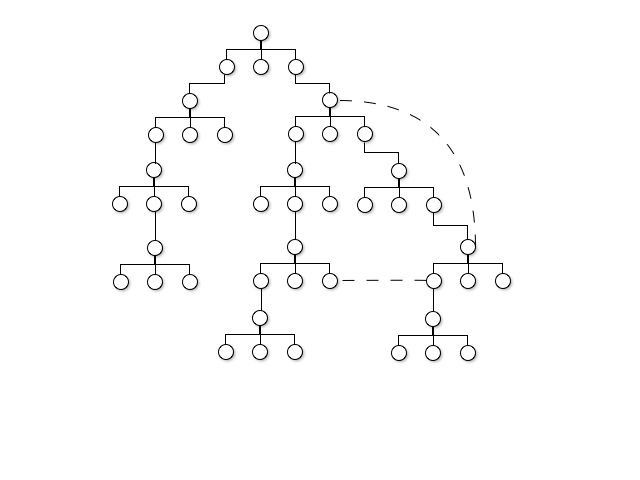
\includegraphics[width=0.5\textwidth]{images/network}
  \caption{Representative lateral and hierarchical cycles.}
  \label{fig:network}
\end{figure}

\subsubsection{Hierarchical Movement of Data}
The establishment of temporary connectivity from one echelon to another, which bypasses the standard chain of command can also result in a hierarchical movement of data.  Such situation may exist if, for example, a Company Commander required a Sat-Com link to a Division asset or if that Commander (or his staff) travels to Division HQ.  In both cases we are creating network cycles in the form of temporary links that transcend the hierarchical structure of the graph and connect nodes that are otherwise separated by much larger geodesic distances.  This has a nontrivial effect\cite{Ganesh:2005} on rate at which data is disseminated across the network.


\section{Disaster Recovery}
\label{sec:dr}
An event in which a node suffers catastrophic loss of data, characterized as a disaster recovery scenario, can be evaluated with epidemic modeling.  In both cases there is a non-trivial healing function which occurs over some $t$ time steps and which is affected by the network topology\cite{Ganesh:2005}.  In the former case, the disaster recovery \emph{heals} similar to a standard S-I-R model.  The failed node is analogous to the infected state (as in a cellular automata).  As the data propagates back, the infected node transitions to a recovered state.  All nodes on the network are assumed to be susceptible.  

As with all data flow on the network, the rate of propagation of data to the failed node is determined by bandwidth and probability of connectivity, both of which have been previously defined in terms of their geodesic distance to the root node.  A complete discussion of this additional modeling is left to future work.


\section{Related Work}
\label{sec:related}
Given the rapidly evolving nature of both military conflict and technology, there are many opportunities to extend and enhance this work.  Possibilities for additional related work include the following.

Individual datum may have different levels of importance, and consequently there may be the need to address QoS issues on the network.  In the context investigated in this paper, all data are treated equally on the network and there is no attempt made to differentiate datum, sender, or recipient, although all three might be a valid basis for establishing precedence.

Especially in a military context, but in others as well, there is a need to control access to data based on different criteria.  Frequently this takes the form of an access list or is managed through credentials during sign-on.  Security has been summarily ignored for the sake of this discussion, but must be implemented in a way that satisfies the needs of the organization.  In many situations this extends not only to controlling data access by individuals on the network but also controlling what data reaches the network in the first place.  In the military this is sometimes referred to as a red-black issue and much of the concern over security revolves around defending network borders.
	
In Section \ref{sec:doe} we briefly mentioned dynamic distributed federated databases (DDFDs) and suggested that there might at some future point be an opportunity to assess their fitness for use in austere conditions.  They are popular and will become a viable solution as network capacity and reliability continue to increase or where data needs are sufficiently localized and local connectivity allows.


\section{Summary}
\label{sec:conclusion}
We discovered that we can rely on the established hierarchical structure, alone, to ensure that data on the network will converge to a stable consistent state.  Furthermore, we find that this will occur in polynomial time roughly proportional to $O(n^{2})$ in the worst case, although it will likely approach $O(n)$.  

The interesting finding, though, is that the introduction of a relatively small number of cycles significantly speeds up the process of data synchronization\cite{Watts:1998}.  Given a sufficiently high probability of cycle creation, we can expect federation in time proportional to no greater than $O(n)$ and more likely approaching $O(log(n))$.


\newpage
\section*{Acknowledgment}
The authors would like to thank Dr. Timothy Chung and the Systems Engineering Department of the Naval Postgraduate School for their support, resources, and motivation.


% references
\bibliographystyle{IEEEtran}
\bibliography{../../581Thesis/bibtex/581}
%The following is just a collection of citations that may (or may not) be used in this paper.  I have collected them here in order to ensure they not get misplaced.
%\cite{Hui:2011}\cite{Liu:2009}\cite{Vahdat:2000}\cite{Gross:2006}\cite{Fu:2003}\cite{Ganesh:2005}
%\cite{Bent2009}\cite{Bent:2008}\cite{Toce:2011}\cite{Sonnenberg:2009}\cite{Watts:1998}


\end{document}


